\begin{figure}[!h]
    \centering
    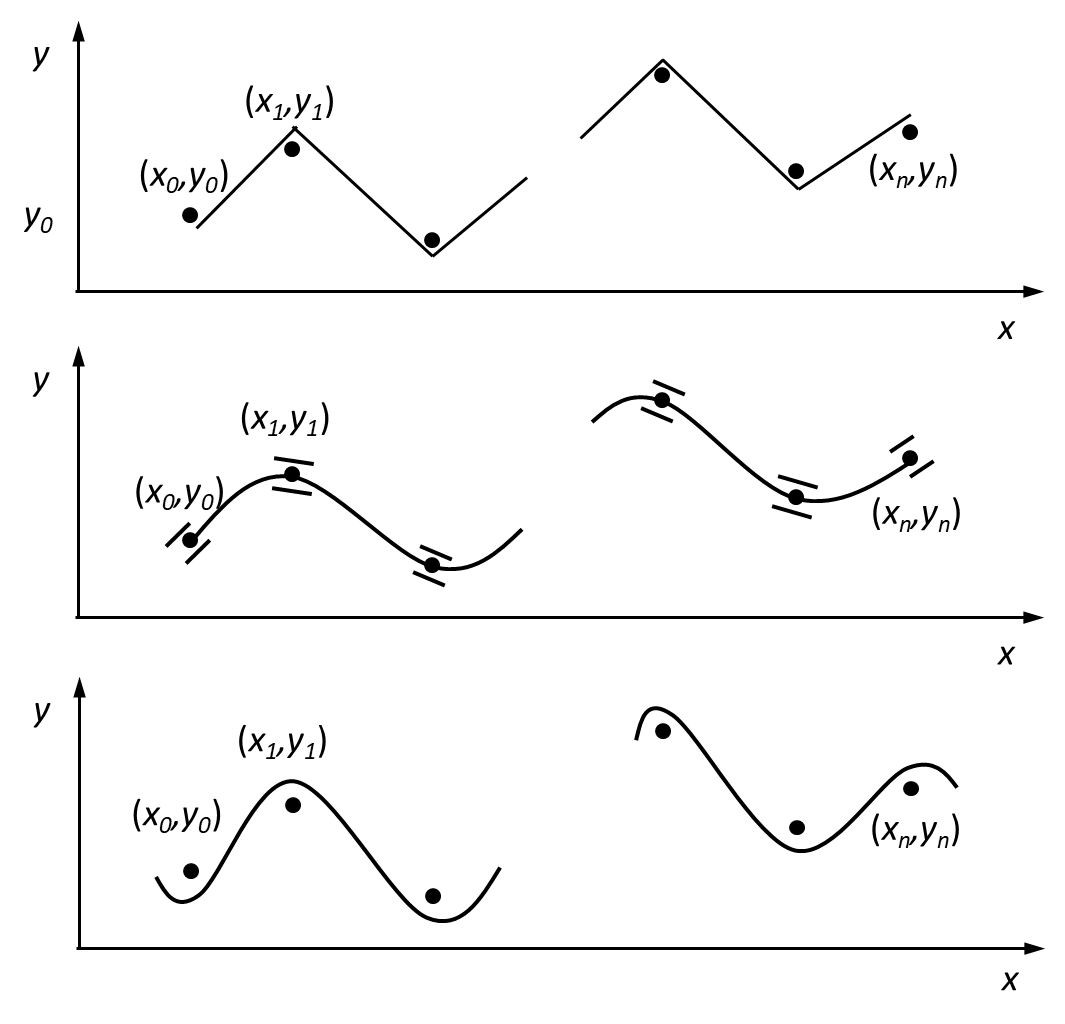
\includegraphics[width=.8\textwidth]{figures/phys_spline.png}
    \caption{Гладкая кусочно-кубическая интерполяция. $u(x)$ - исходная функция $U(x)$ - сплайн третьей степени}
\end{figure}

Самыми распространенными являются кубические сплайны, имеющие имеют вид:
\begin{equation}
    S_3 (x) = P_{3,i} (x) = a_i + b_i (x-x_i) + \frac{c_i}{2} (x-x_i)^2 + \frac{d_i}{6}(x-x_i)^3 \textup{ на } [x_{i-1},x_i]
    \label{Eq:spline_3}
\end{equation}
\begin{equation*}
    P_{3,i} (x_{i-1} )=y_{i-1},\   P_{3,i} (x_i) = y_i,\ i=1 \dots n
\end{equation*}

Форма записи \eqref{Eq:spline_3} соответствует ряду Тейлора для $P_{3,i}$ в окрестности точки $x_i$, и она позволяет заключить, что 
\begin{equation*}
    a_i = P_{3,i} (x_i),\ b_i = P_{3,i}' (x_i),\ 
    c_i = P_{3,i}'' (x_i),\ d_i = P_{3,i}''' (x_i)
\end{equation*}

Однако, система \eqref{Eq:spline_3} задана двумя уравнениями относительно четырех неизвестных $a_i,b_i,c_i,d_i$, И чтобы решить ее, необходимо получить еще два уравнения для каждого промежутка $[x_{i-1},x_i]$.
Сделать это можно двумя способами.